%Este trabalho está licenciado sob a Licença Atribuição-CompartilhaIgual 4.0 Internacional Creative Commons. Para visualizar uma cópia desta licença, visite http://creativecommons.org/licenses/by-sa/4.0/deed.pt_BR ou mande uma carta para Creative Commons, PO Box 1866, Mountain View, CA 94042, USA.

\chapter{Limites}\label{cap_lim}
\thispagestyle{fancy}

\section{Noção de limites}\label{cap_lim_sec_lim}

Seja $f$ uma função definida em um intervalo aberto em torno de um dado ponto $x_0$, exceto talvez em $x_0$. Quando o valor de $f(x)$ é arbitrariamente próximo de um número $L$ para $x$ suficientemente próximo de $x_0$, escrevemos
\begin{equation}
  \lim_{x\to x_0} f(x) = L
\end{equation}
e dizemos que o limite da função $f$ é $L$ quando $x$ tende a $x_0$.

\begin{ex}\label{ex:lim0}
  Consideremos a função
  \begin{equation}
    f(x) = \frac{(x^2-1)(x-2)}{(x-1)(x-2)}.
  \end{equation}
  Na Figura \ref{fig:ex_lim0}, temos um esboço do gráfico desta função.

  \begin{figure}[H]
    \centering
    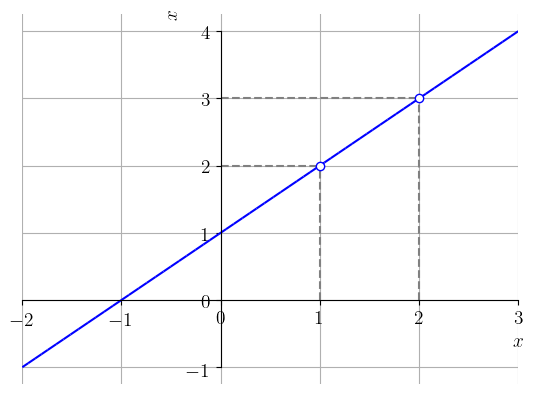
\includegraphics[width=0.7\textwidth]{./cap_lim/dados/fig_ex_lim0/fig_ex_lim0}
    \caption{Esboço do gráfico da função $f(x)$ dada no Exemplo \ref{ex:lim0}.}
    \label{fig:ex_lim0}
  \end{figure}


  Vejamos os seguintes casos:
  \begin{itemize}
  \item $\displaystyle \lim_{x\to 0} f(x) = 1 = f(0)$.
    
    \begin{tabular}{r|ccc|c|ccc}
      $x$ & $-0,01$ & $-0,001$ & $-0,0001$ & $\rightarrow 0 \leftarrow$ & $0,0001$ & $0,001$ & $0,01$\\\hline
      $f(x)$ & $0,99$ & $0,999$ & $0,9999$ & $\rightarrow 1 \leftarrow$ & $0,0001$ & $0,001$ & $0,01$
    \end{tabular}

    \ifispython
    No \verb+SymPy+, podemos computar este limite com o comando
\begin{verbatim}
limit((x**2-1)*(x-2)/((x-1)*(x-2)),x,0)
\end{verbatim}
    \fi
  \item $\displaystyle \lim_{x\to 1} f(x) = 2$, embora $f(1)$ não esteja definido.
    
    \begin{tabular}{r|ccc|c|ccc}
      $x$ & $0,9$ & $0,99$ & $0,999$ & $\rightarrow 1 \leftarrow$ & $1,0001$ & $1,001$ & $1,01$\\\hline
      $f(x)$ & $1,9$ & $1,99$ & $1,999$ & $\rightarrow 2 \leftarrow$ & $2,0001$ & $2,001$ & $2,01$
    \end{tabular}
  \item $\displaystyle \lim_{x\to 2} f(x) = 3$, embora $f(2)$ também não esteja definido. Verifique!
  \end{itemize}
\end{ex}

\subsection{Limites da função constante e da função identidade}

Da noção de limite, temos
\begin{equation}
  \lim_{x\to x_0} k = k,
\end{equation}
seja qual for a constante $k$. Vejamos a Figura \ref{fig:lim_funk}.

\begin{figure}[H]
  \centering
  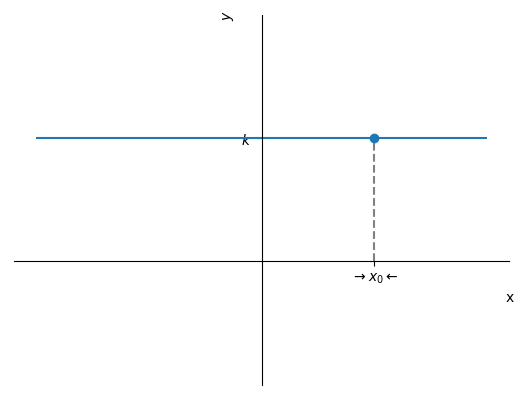
\includegraphics[width=0.7\textwidth]{./cap_lim/dados/fig_lim_funk/fig_lim_funk}
  \caption{Esboço do gráfico de uma função constante $f(x) = k$.}
  \label{fig:lim_funk}
\end{figure}

Também da noção de limites, podemos inferir que
\begin{equation}
  \lim_{x\to x_0} x = x_0,
\end{equation}
seja qual for o ponto $x_0$. Vejamos a Figura \ref{fig:lim_funid}.

\begin{figure}[H]
  \centering
  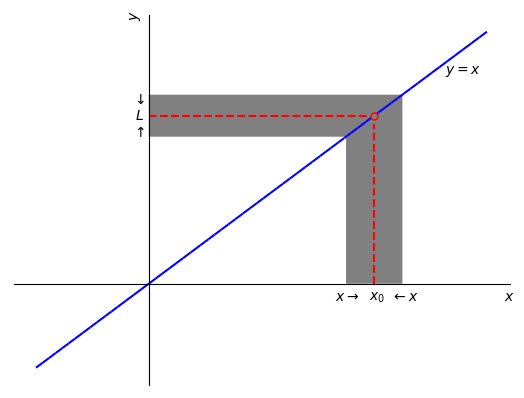
\includegraphics[width=0.7\textwidth]{./cap_lim/dados/fig_lim_funid/fig_lim_funid}
  \caption{Esboço do gráfico da função identidade $f(x) = x$.}
  \label{fig:lim_funid}
\end{figure}

\subsection*{Exercícios}

\begin{exer}\label{exer:limgraf}
  Considere que uma dada função $f$ tenha o seguinte esboço de gráfico:
  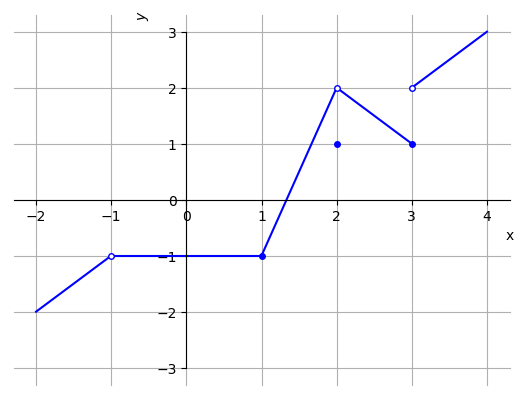
\includegraphics[width=0.8\textwidth]{./cap_lim/dados/fig_exer_limgraf/fig_exer_limgraf}

  Forneça o valor dos seguintes limites:
  \begin{enumerate}[a)]
  \item $\displaystyle \lim_{x\to -1} f(x)$
  \item $\displaystyle \lim_{x\to 1} f(x)$
  \item $\displaystyle \lim_{x\to 2} f(x)$
  \item $\displaystyle \lim_{x\to 2} f(x)$
  \item $\displaystyle \lim_{x\to 3} f(x)$
  \end{enumerate}
\end{exer}
\begin{resp}
  a)~$-1$; b)~$-1$; c)~$2$; d)~$\nexists$
\end{resp}

\begin{exer}
  Considerando a mesma função do exercício anterior (Exercícios \ref{exer:limgraf}), forneça
  \begin{enumerate}
  \item $\displaystyle \lim_{x\to -\frac{3}{2}} f(x)$
  \item $\displaystyle \lim_{x\to 0} f(x)$
  \item $\displaystyle \lim_{x\to \frac{3}{4}} f(x)$
  \end{enumerate}
\end{exer}

\emconstrucao

\section{Regras para o cálculo de limites}\label{cap_lim_sec_regras}

Sejam dados os seguintes limites
\begin{equation}
  \lim_{x\to x_0} f(x) = L_1\qquad\text{e}\qquad \lim_{x\to x_0} g(x) = L_2,
\end{equation}
com $x_0, L_1, L_2$ números reais. Então, valem as seguintes regras:
\begin{itemize}
\item Regra da multiplicação por um escalar:
  \begin{equation}
    \lim_{x\to x_0} kf(x) = k\lim_{x\to x_0} f(x) = kL_1,
  \end{equation}
  para qualquer número real $k$.
\item Regra da soma:
  \begin{equation}
    \lim_{x\to x_0} f(x) + g(x) = \lim_{x\to x_0} f(x) + \lim_{x\to x_0} g(x) = L_1 + L_2
  \end{equation}
\item Regra do produto:
  \begin{equation}
    \lim_{x\to x_0} f(x) \cdot g(x) = \lim_{x\to x_0} f(x) \cdot \lim_{x\to x_0} g(x) = L_1 \cdot L_2
  \end{equation}
\item Regra do quociente:
  \begin{equation}
    \lim_{x\to x_0} \frac{f(x)}{g(x)} = \frac{\lim_{x\to x_0} f(x)}{\lim_{x\to x_0} g(x)} = \frac{L_1}{L_2},
  \end{equation}
  desde que $L_2\neq 0$.
\item Regra da potenciação:
  \begin{equation}
    \lim_{x\to x_0} (f(x))^s = L_1^s,
  \end{equation}
  se $L_1^s$ é um número real. 
\end{itemize}

Podemos usar essas regras para calcularmos limites.

\begin{ex}
  Vejamos os seguintes casos:
  \begin{enumerate}[a)]
  \item $\displaystyle \lim_{x\to -1} 2x$
  \begin{align}
    \lim_{x\to -1} 2x &= 2\lim_{x\to -1} x\\
    &= 2\cdot(-1) = -2
  \end{align}
  \ifispython
  No \verb+SymPy+, podemos computar este limite com
\begin{verbatim}
limit(2*x,x,-1)
\end{verbatim}
  \fi
\item $\displaystyle \lim_{x\to 2} x^2 - 1$
  \begin{align}
    \lim_{x\to 2} x^2 - 1 &= \lim_{x\to 2} x^2 - \lim_{x\to 2} 1\\
                          &= \left(\lim_{x\to 2} x\right)^2 - \lim_{x\to 2} 1\\
    &= 2^2 - 1 = 3.
  \end{align}
  \ifispython
  No \verb+SymPy+, podemos computar este limite com
\begin{verbatim}
limit(x**2-1,x,-1)
\end{verbatim}
  \fi
\item $\displaystyle \lim_{x\to -1} \sqrt{1-x^2}$.
  \begin{align}
    \lim_{x\to -1} \sqrt{1-x^2} &= \sqrt{\lim_{x\to -1} 1-x^2}\\
                                &= \sqrt{\lim_{x\to -1} 1 - \left(\lim_{x\to -1} x\right)^2}\\
                                &= \sqrt{1 - (-1)^2} \\
                                &= 0.
  \end{align}
  \ifispython
  No \verb+SymPy+, podemos computar este limite com
\begin{verbatim}
limit(sqrt(1-x**2),x,-1)
\end{verbatim}
  \fi  
\item $\displaystyle \lim_{x\to 0} \frac{(x^2-1)(x-2)}{(x-1)(x-2)}$
  \begin{align}
    \lim_{x\to 0} \frac{(x^2-1)(x-2)}{(x-1)(x-2)} &= \frac{\lim_{x\to 0}(x^2-1)(x-2)}{\lim_{x\to 0} (x-1)(x-2)}\\
                                                  &= \frac{\lim_{x\to x_0} (x^2-1)\lim_{x\to 0}(x-2)}{\lim_{x\to 0}(x-1)\lim_{x\to 0}(x-2)}\\
    &= \frac{-2}{-2} = 1.
  \end{align}
  \end{enumerate}
\end{ex}

\begin{prop}\normalfont{(Limites de polinômios)}\label{prop:lim_poli}
  Se $p(x) = a_nx^n + a_{n-1}x^{n-1} + \cdots + a_0$, então
  \begin{equation}
    \lim_{x\to b} p(x) = p(b) = a_nb^n + a_{n-1}b^{n-1} + \cdots + a_0,
  \end{equation}
  para qualquer número real $b$ dado.
\end{prop}
\begin{dem}
  Segue das regras da soma, da multiplicação por escalar e da potenciação. Vejamos
  \begin{align}
    \lim_{x\to b} p(x) &= \lim_{x\to b} a_nx^n + a_{n-1}x^{n-1} + \cdots + a_0\\
                       &= \lim_{x\to b} a_nx^n + \lim_{x\to b} a_{n-1}x^{n-1} + \cdots + \lim_{x\to b} a_0\\
                       &= a_n\left(\lim_{x\to b} x\right)^n + a_{n-1}\left(\lim_{x\to b} x\right)^{n-1} + \cdots + a_0\\
                       &= a_nb^n + a_{n-1}b^{n-1} + \cdots + a_0 = p(b).
  \end{align}
\end{dem}

\begin{ex}
  \begin{equation}
    \lim_{x\to \sqrt{2}} 2x^4 - 2x^2 + x = 2(\sqrt{2})^4 - 2(\sqrt{2})^2 + \sqrt{2} = 4+\sqrt{2}.
  \end{equation}
  \ifispython
  No \verb+SymPy+, podemos computar este limite com o comando
\begin{verbatim}
limit(2*x**4-2*x**2+x,x,sqrt(2))
\end{verbatim}
  \fi
\end{ex}

\begin{prop}\normalfont{(Limite de funções racionais)}
  Sejam $r(x) = p(x)/q(x)$ é uma função racional e $b$ um número real tal que $q(b)\neq 0$. Então,
  \begin{equation}
    \lim_{x\to b} \frac{p(x)}{q(x)} = \lim_{x\to b} \frac{p(b)}{q(b)}.
  \end{equation}
\end{prop}
\begin{dem}
  Segue da regra do limite do quociente e da Proposição \ref{prop:lim_poli}:
  \begin{align}
    \lim_{x\to b} \frac{p(x)}{q(x)} &= \frac{\lim_{x\to b} p(x)}{\lim_{x\to b} q(x)} \\
    &= \frac{p(b)}{q(b)}.
  \end{align}
\end{dem}

\begin{ex}
  \begin{equation}
    \lim_{x\to 0} \frac{(x^2-1)(x-2)}{(x-1)(x-2)} = \frac{(0^2-1)(0-2)}{(0-1)(0-2)} = 1.
  \end{equation}
\end{ex}

\subsection{Indeterminação $0/0$}

Quando $f(a)=0$ e $g(a)=0$, dizemos que
\begin{equation}
  \lim_{x\to a} \frac{f(x)}{g(x)}
\end{equation}
é uma indeterminação do tipo $0/0$. Em vários destes casos, podemos calcular o limite eliminando o fator em comum $(x-a)$.

\begin{ex}
  \begin{align}
    \lim_{x\to 2}\frac{(x^2-1)(x-2)}{(x-1)(x-2)} = \lim_{x\to 2} \frac{x^2-1}{x-1} = 3.
  \end{align}
  \ifispython
  No \verb+SymPy+, podemos computar o limite acima com
\begin{verbatim}
limit((x**2-1)*(x-2)/((x-1)*(x-2)),x,2)
\end{verbatim}
  \fi
\end{ex}

Quando o fator em comum não aparece explicitamente, podemos tentar trabalhar algebricamente de forma a explicitá-lo.

\begin{ex}
  No caso do limite
  \begin{align}
    \lim_{x\to 1} \frac{x^3-3x^2-x+3}{x^2+x-2}
  \end{align}
  temos que o denominador $p(x) = x^3-3x^2-x+3$ se anula em $x=1$, assim como o denominador $q(x) = x^2+x-2$. Assim sendo, $(x-1)$ é um fator em comum entre $p(x)$ e $q(x)$. Para explicitá-lo, 
  \begin{equation}
    \frac{p(x)}{x-1} = x^2-2x-3\qquad\text{e}\qquad\frac{q(x)}{x-1} = x+2.
  \end{equation}
  \ifispython
  No \verb+SymPy+, podemos computar estas divisões com os seguintes comandos
\begin{verbatim}
simplify((x**3-3*x**2-x+3)/(x-1))
simplify((x**2+x-2)/(x-1))
\end{verbatim}
  \fi
  Realizadas as divisões, temos
  \begin{equation}
    p(x) = (x-1)(x^2-2x-3)\qquad\text{e}\qquad q(x)=(x-1)(x+2).
  \end{equation}
  Com isso, temos
  \begin{align}
    \lim_{x\to 1} \frac{x^3-3x^2-x+3}{x^2+x-2} &= \lim_{x\to 1} \frac{(x-1)(x^2-2x-3)}{(x-1)(x+2)} \\
    &- \lim_{x\to 1} \frac{x^2-2x-3}{x+2} = -\frac{4}{3}.
  \end{align}
\end{ex}

\begin{ex}
  No caso de
  \begin{equation}
    \lim_{x\to 0} \frac{\sqrt{1-x}-1}{x}
  \end{equation}
  temos uma indeterminação do tipo $0/0$ envolvendo uma raiz. Neste caso, podemos calcular o limite usando de racionalização
  \begin{align}
    \lim_{x\to 0} \frac{\sqrt{1-x}-1}{x} &= \lim_{x\to 0} \frac{\sqrt{1-x}-1}{x}\frac{\sqrt{1-x}+1}{\sqrt{1-x}+1}\\
                                         &= \lim_{x\to 0} \frac{1-x-1}{x(\sqrt{1-x}+1)} \\
                                         &- \lim_{x\to 0} \frac{-x}{x(\sqrt{1-x}+1)}\\
    &= \lim_{x\to 0} \frac{-1}{\sqrt{1-x}+1} = -\frac{1}{2}.
  \end{align}
  \ifispython
  Com o \verb+SymPy+, podemos computar este limite com
\begin{verbatim}
limit((sqrt(1-x)-1)/x,x,0)
\end{verbatim}
  \fi
\end{ex}

\subsection*{Exercícios}

\begin{exer}
  Assumindo que o $\lim_{x\to 2} f(x) = L$ e que
  \begin{equation}
    \lim_{x\to 2} \frac{f(x)-2}{x+2} = 1,
  \end{equation}
  forneca o valor de $L$.
\end{exer}
\begin{resp}
  $6$
\end{resp}
\emconstrucao

\section{Limites laterais}\label{cap_lim_sec_lateral}

Seja dada uma função $f$ definida para todo $x$ em um intervalo aberto $(L, a)$, sendo $a$ um número real com $L<a$ podendo ser $L=-\infty$. O {\bf limite lateral à esquerda} de $f$ no ponto $a$ é denotado por
\begin{equation}
  \lim_{x\to a^-} f(x)
\end{equation}
e é computado tendo em vista a tendência da função apenas para pontos $x<a$. Em outras palavras, o
\begin{equation}
  \lim_{x\to a^-} f(x) = L
\end{equation}
quando $f(x)$ pode ser tomado arbitrariamente próximo de $L$, desde que tomemos $x<a$ suficientemente próximo de $a$.

Para uma função $f$ definida para todo $x$ em um intervalo aberto $(a, L)$, sendo $a$ um número real com $L>a$ podendo ser $L=\infty$, o {\bf limite lateral à direita} de $f$ no ponto $a$ é denotado por
\begin{equation}
  \lim_{x\to a^+} f(x)
\end{equation}
e é computado tendo em vista a tendência da função apenas para pontos $x>a$. Em outras palavras, temos
\begin{equation}
  \lim_{x\to a^+} f(x) = L,
\end{equation}
quando $f(x)$ pode ser tomado arbitrariamente próximo de $L$, desde que tomemos $x>a$ suficientemente próximo de $a$.

\begin{obs}
  Por inferência direta, temos
  \begin{equation}
    \lim_{x\to a^{\pm}} k = k\quad\text{e}\quad\lim_{x\to a^{\pm}} x = a^{\pm},
  \end{equation}
  onde $a$ e $k$ são quaisquer números reais.
\end{obs}

\begin{exer}\label{ex:lim_absx}
  Vamos calcular
  \begin{equation}
    \lim_{x\to 0^-} |x|.
  \end{equation}
  Por definição, temos
  \begin{equation}
    |x| := \left\{
      \begin{array}{ll}
        x &, x\geq 0,\\
        -x &, x< 0.
      \end{array}
    \right.
  \end{equation}
  Como estamos interessados no limite lateral à esquerda de $x=0$, trabalhamos com $x<0$ e, então
  \begin{equation}
    \lim_{x\to 0^-} |x| = \lim_{x\to 0^-} -x = -\lim_{x\to 0^-} x = 0.
  \end{equation}
  
  Analogamente, calculamos
  \begin{equation}
    \lim_{x\to 0^+} |x| = \lim_{x\to 0^+} x = 0.
  \end{equation}
  Verifique!

  \ifispython
  Usando o \verb+SymPy+, podemos computar os limites acima com os seguintes comandos:
\begin{verbatim}
limit(abs(x),x,0,'-')
limit(abs(x),x,0,'+')
\end{verbatim}
  \fi
\end{exer}

\begin{teo}\label{teo:lim_existe}
  Existe o limite de uma dada função $f$ no ponto $x=a$ e $\lim_{x\to a} f(x) = L$ se, e somente se, existem e são iguais a $L$ os limites laterais à esquerda e à direita de $f$ no ponto $x=a$.
\end{teo}

\begin{exer}
  No exemplo anterior (Exemplo \ref{ex:lim_absx}), vimos que
  \begin{equation}
    \lim_{x\to 0^-} |x| = \lim_{x\to 0^+} |x| = 0.
  \end{equation}
  Logo, pelo teorema acima (Teorema \ref{teo:lim_existe}), podemos concluir que
  \begin{equation}
    \lim_{x\to 0} |x| = 0.
  \end{equation}
\end{exer}

\begin{exer}
  Vamos verificar a existência de
  \begin{equation}
    \lim_{x\to 0} \frac{|x|}{x}.
  \end{equation}
  Começamos pelo limite lateral à esquerda, temos
  \begin{align}
    \lim_{x\to 0^-} \frac{|x|}{x} &= \lim_{x\to 0^-} \frac{-x}{x}\\
    &= \lim_{x\to 0^-} -1 = -1.
  \end{align}
  Agora, calculando o limite lateral à direta, obtemos
  \begin{align}
    \lim_{x\to 0^+} \frac{|x|}{x} &= \lim_{x\to 0^+} \frac{x}{x}\\
    &= \lim_{x\to 0^+} 1 = 1.
  \end{align}
  Como os limites laterais à esquerda e à direita são diferentes, concluímos que não existe o limite de $|x|/x$ no ponto $x=0$.

  \ifispython
  No \verb+Sympy+, por padrão o limite computado é sempre o limite lateral à direita. É por isso que o comando
\begin{verbatim}
limit(abs(x)/x,x,0)
\end{verbatim}
  fornece o valor $1$ como saída.
  \fi
\end{exer}

\subsection*{Exercícios}

\emconstrucao

\section{Limites e desigualdades}\label{cap_lim_sec_limdes}

Se $f$ e $g$ são funções tais que $f(x)<g(x)$ para todo $x$ em um certo intervalo aberto contendo $a$, exceto possivelmente em $x=a$, e existem os limites de $f$ e $g$ no ponto $x=a$, então
\begin{equation}
  \lim_{x\to a} f(x) \leq \lim_{x\to a} g(x).
\end{equation}
Observe que a tomada do limite não preserva a desigualdade estrita.

\begin{exer}
  As funções $f(x) = x^2/3$ e $g(x) = x^2/2$ são tais que $f(x) < g(x)$ para todo $x\neq 0$. Ainda, temos
  \begin{equation}
    \lim_{x\to 0} f(x) = 0\quad\text{e}\quad\lim_{x\to 0} g(x) = 0.
  \end{equation}
\end{exer}

\begin{obs}
  A preservação da desigualdade também ocorre para limites laterais. Mais precisamente, se $f$ e $g$ são funções tais que $f(x)<g(x)$ para todo $x < a$ e existem os limites lateral à esquerda de $f$ e $g$ no ponto $x=a$, então
  \begin{equation}
    \lim_{x\to a^-} f(x) \leq \lim_{x\to a^-} g(x).
  \end{equation}
  Vale o resultado análogo para limite lateral à direito. Escreva-o!
\end{obs}

\subsection{Teorema do confronto}

\begin{teo}\normalfont{(Teorema do confronto)}\label{teo:confronto}
  Se $g(x) \leq f(x) \leq h(x)$ para todo $x$ em um intervalo aberto contendo $a$, exceto possivelmente em $x=a$, e
  \begin{equation}
    \lim_{x\to a} g(x) = \lim_{x\to a} h(x) = L,
  \end{equation}
  então
  \begin{equation}
    \lim_{x\to a} f(x) = L.
  \end{equation}
\end{teo}
\begin{dem}
  Da preservação da desigualdade, temos
  \begin{equation}
    \lim_{x\to a} g(x) \leq \lim_{x\to a} f(x) \leq \lim_{x\to a} h(x)
  \end{equation}
  donde
  \begin{equation}
    L \leq \lim_{x\to a} f(x) \leq L.
  \end{equation}
\end{dem}

\begin{exer}
  Toda função $f(x)$ tal que $-1+x^2/2 \leq f(x) \leq -1+x^2/3$, para todo $x\neq 0$, tem
  \begin{equation}
    \lim_{x\to 0} f(x) = -1.
  \end{equation}
\end{exer}

\begin{obs}
  O Teorema do confronto também se aplica a limites laterais.
\end{obs}

\begin{ex}\label{ex:senx}
  \begin{equation}
    \lim_{x\to 0} \sen x = 0.
  \end{equation}
  De fato, começamos assumindo $0<x<\pi/2$. Tomando $O = (0,0)$, $A=(1,0)$ e $P = (\cos x, \sen x)$, observamos que
  \begin{equation}
    \text{Área do triâng.} OAP < \text{Área do setor} OAP,
  \end{equation}
  i.e.
  \begin{equation}
    \frac{\sen x}{2} < \frac{x}{2} \Rightarrow \sen x < x,
  \end{equation}
  para todo $0< x < \pi/2$. 

  É certo que $\sen x < -x$ para $-\pi/2 < x < 0$. Com isso e o resultado acima, temos
  \begin{equation}\label{eq:senx0}
    \sen x \leq |x|,\quad -\pi/2 < x < \pi/2.
  \end{equation}

  Lembrando que $\sen x$ é uma função ímpar, temos
  \begin{equation}\label{eq:senx1}
    -|x| \leq -\sen x = \sen -x,\quad -\pi/2 < x < \pi/2.
  \end{equation}
  Logo, de \eqref{eq:senx0} e \eqref{eq:senx1}, temos
  \begin{equation}
    -|x| \leq \sen x \leq |x|.
  \end{equation}

  Por fim, como
  \begin{equation}
    \lim_{x\to 0} -|x| = \lim_{x\to 0} |x| = 0,
  \end{equation}
  do Teorema do confronto, concluímos
  \begin{equation}
    \lim_{x\to 0} \sen x = 0.
  \end{equation}
\end{ex}

\begin{obs}
  Do exemplo anterior (Exemplo \ref{ex:senx}), podemos mostrar que
\begin{equation}
  \lim_{x\to 0} \cos x = 1.
\end{equation}

De fato, da identidade trigonométrica de ângulo metade \eqref{eq:id_trig_cos_x2}
\begin{equation}
  \sen^2 \frac{x}{2} = \frac{1 - \cos x}{2}
\end{equation}
temos
\begin{equation}
  \cos x = 1 + 2\sen^2 \frac{x}{2}.
\end{equation}
Então, aplicando as regras de cálculo de limites, obtemos
\begin{align}
  \lim_{x\to 0} \cos x &= \lim_{x\to 0} \left[1 + 2\sen^2 \frac{x}{2}\right] \\
                       &= 1 + 2\left(\lim_{x\to 0} \sen \frac{x}{2}\right)^2.\label{eq:senx2}
\end{align}
Agora, fazemos a mudança de variável $y = x/2$. Neste caso, temos $y\to 0$ quando $x\to 0$ e, então
\begin{equation}
  \lim_{x\to 0} \sen \frac{x}{2} = \lim_{y\to 0} \sen y = 0.
\end{equation}
Então, retornando a equação \eqref{eq:senx2}, concluímos
\begin{equation}
  \lim_{x\to 0} \cos x = 1.
\end{equation}
\end{obs}

\subsection{Limites envolvendo $(\sen x)/x$}

Verificamos o seguinte resultado
\begin{equation}
  \lim_{x\to 0} \frac{\sen x}{x} = 1.
\end{equation}

Para verificarmos este resultado, calcularemos os limites laterais à esquerda e à direita. Começamos com o limite lateral a direita e assumimos $0<x<\pi/2$. Sendo os pontos $O=(0,0)$, $P=(\cos x,\sen x)$, $A = (1,0)$ e $T = (1, \tg x)$, observamos que
\begin{equation}
  \text{Área do triâng. } OAP < \text{Área do setor} OAP < \text{Área do triâng. } OAT.
\end{equation}
Ou seja, temos
\begin{equation}
  \frac{\sen x}{2} < \frac{x}{2} < \frac{\tg x}{2}.
\end{equation}
Multiplicando por $2$ e dividindo por $\sen x$\footnote{$\sen x > 0$ para todo $0< x < \pi/2$.}, obtemos
\begin{equation}
  1 < \frac{x}{\sen x} < \frac{1}{\cos x}.
\end{equation}
Tomando os recíprocos, temos
\begin{equation}
  1 > \frac{\sen x}{x} > \cos x.
\end{equation}
Agora, passando ao limite
\begin{equation}
  1 = \lim_{x\to 0^+} 1 \geq \lim_{x\to 0^+} \frac{\sen x}{x} \geq \lim_{x\to 0^+} \cos x = 1.
\end{equation}
Logo, concluímos que
\begin{equation}
  \lim_{x\to 0^+} \frac{\sen x}{x} = 1.
\end{equation}

Agora, usando o fato de que $\sen x/x$ é uma função par, temos
\begin{align}
  \lim_{x\to 0^-} \frac{\sen x}{x} &= \lim_{x\to 0^-} \frac{\sen(-x)}{-x} \\
  &= \lim_{x\to 0^+} \frac{\sen x}{x} = 1.
\end{align}

Calculados os limites laterais, concluímos o que queríamos.

\begin{ex}
  Com o resultado acima e as regras de cálculo de limites, temos
  \begin{equation}
    \lim_{x\to 0} \frac{\cos(x) - 1}{x} = 0.
  \end{equation}
  Veja o Exercício \ref{exer:lim_cosx_1}.
\end{ex}

% \begin{exer}
%   Pode-se mostrar que $|-x| \leq \sen x \leq |x|$ (veja a Figura \ref{fig:}). Ainda, como
%   \begin{equation}
%     \lim_{x\to 0} -|x| = \lim_{x\to 0} |x| = 0,
%   \end{equation}
%   temos, pelo Teorema do confronto (Teorema \ref{teo:confronto}),
%   \begin{equation}
%     \lim_{x\to 0} \sen x = 0.
%   \end{equation}
% \end{exer}

\subsection*{Exercícios}

\begin{exer}
  Supondo que $1-x^2/3 \leq u(x) \leq 1-x^2/2$ para todo $x\neq 0$, determine o $\lim_{x\to 0} u(x)$.
\end{exer}
\begin{resp}
  $1$
\end{resp}

\begin{exer}
  Calcule
  \begin{equation}
    \lim_{x\to 0} \frac{\sen 3x}{6x}.
  \end{equation}
\end{exer}
\begin{resp}
  $0$
\end{resp}

\begin{exer}\label{exer:lim_cosx_1}
  Calcule
  \begin{equation}
    \lim_{x\to 0} \frac{\cos(x)-1}{x}.
  \end{equation}
\end{exer}
\begin{resp}
  $0$
\end{resp}

\begin{exer}
  Calcule
  \begin{equation}
    \lim_{x\to 0} \frac{\cos(3x)-1}{6x}.
  \end{equation}
\end{exer}
\begin{resp}
  $\frac{1}{2}$
\end{resp}

\emconstrucao

\section{Limites no infinito}\label{cap_lim_sec_liminf}

\emconstrucao

\subsection*{Exercícios}

\section{Limites infinitos}\label{cap_lim_sec_lim_inf}

\emconstrucao

\subsection*{Exercícios}

\emconstrucao

% \section{Taxas de variação e limites}\label{cap_lim_sec_taxa}

% A {\bf taxa de variação}\index{taxa de variação} de $y=f(x)$ em relação a $x$ no intervalo $[x_1, x_2]$ é
% \begin{equation}
%   \frac{\Delta y}{\Delta x} = \frac{f(x_2)-f(x_1)}{x_2-x_1}.
% \end{equation}

% \begin{ex} Vejamos as seguintes aplicações:
%   \begin{itemize}
%   \item Em 1990 o lucro de uma micro empresa foi de $150$ mil reais e em 1992 foi de $165$ mil reais. Desta forma, temos que a taxa de variação do lucro da empresa foi de
%     \begin{equation}
%       \frac{165 - 150}{1992 - 1990} = 7,5\,\mathrm{ mil reais}/\mathrm{ano}.
%     \end{equation}
%   \item Um carro saio do estacionamento às 14h e chegou no seu destino, 150 km do estacionamento, às 16h. Assim sendo, temos que o carro fez o percurso com uma velocidade média (taxa de variação da distância em relação ao tempo) de
%     \begin{equation}
%       \frac{150-0}{16-14} = 75\,\mathrm{km}/\mathrm{h}.
%     \end{equation}
%   \item A taxa de variação da função $f(x) = 2x+x^2$ no intervalo $[-1, 1]$ é
%     \begin{equation}
%       \frac{\Delta y}{\Delta x} = \frac{f(1)-f(-1)}{1-(-1)} = \frac{3-(-1)}{2} = 2.
%     \end{equation}
%     \ifispython
%     No \verb+SymPy+, podemos computar este último exemplo com o código
% \begin{verbatim}
% f = lambda x: 2*x+x**2
% (f(1)-f(-1))/(1-(-1))
% \end{verbatim}
%     \fi
%   \end{itemize}
% \end{ex}
